\section{Instalador del ambiente de análisis de datos}
%%%%%%%%%%%%%% RESUMEN 5%%%%%%%%%%%%%%%%%%
Uno de los objetivos de este trabajo terminal es permitir al usuario empezar a hacer uso de Big Data de una manera más sencilla y sin demasiadas complicaciones. Por lo que se comenzó el desarrollo de un instalador que simplifique el proceso de puesta en marcha del ambiente de análisis de datos.\\

Si bien, el instalador, en este punto del trabajo terminal se encuentra en una fase aún experimental, logra el cometido de simplificar el proceso de puesta en marcha. Esto puede verse reflejado al comparar el número de pasos que se enuncian en el manual de instalación de Luminus, contra el número de pasos que se siguen al utilizar el instalador.\\

La manera en que el instalador simplifica el proceso de instalación es automatizando algunas tareas que de otra forma el usuario tendría que realizar una a una.\\

\subsection{Diagrama de flujo}
\begin{figure}[H]
	\hypertarget{fig:diagramaFlujo}{\hspace{1pt}}
	\begin{center}
		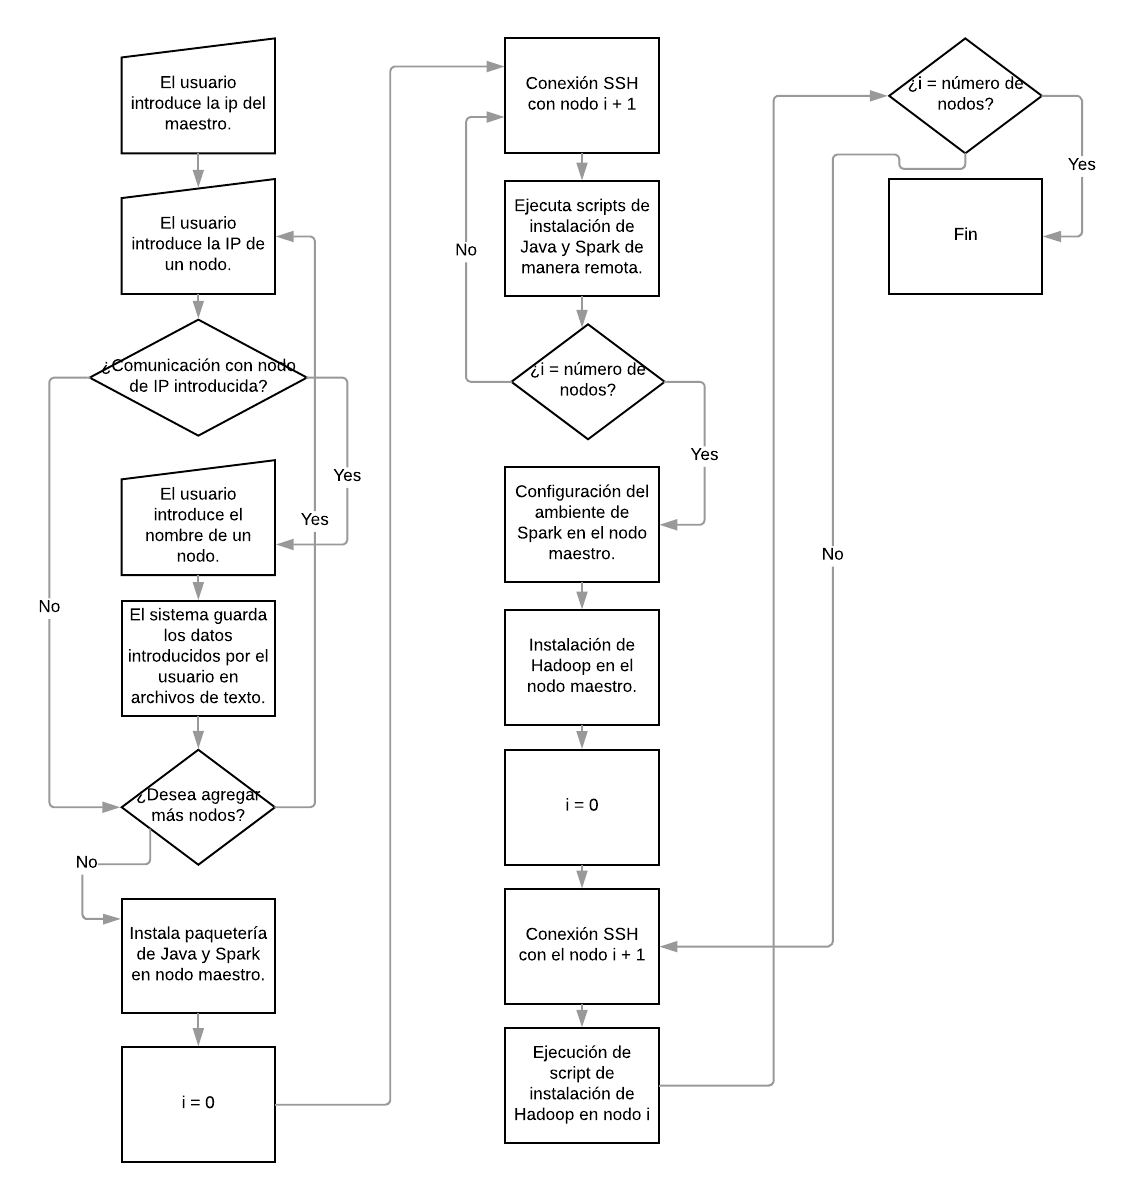
\includegraphics{capitulo5/images/diagramaFlujo.png}
		\caption{Diagrama de flujo de los pasos básicos que sigue el instalador.}
	\end{center}
\end{figure}

